
The zero vector space, $0$, is the vector space which only has one element in it. 
\begin{exercise}
	Let $V_1$ and $V_2$ be vector spaces.
	Suppose that $f: V_1\to V_2$ is a linear map. 
	Show that $\ker(f)=\{0\}$ if and only if the map $f: V_1\to V_2$ is injective.
\end{exercise}

\begin{exercise}Suppose we have 5 vectors spaces and maps between them. 
	\[
		\begin{tikzcd}
			V^0\arrow{r}{d^0} & V^1 \arrow{r}{d^1} & V^2\arrow{r}{d^2} & V^3 \arrow{r}{d^3} & V^4
		\end{tikzcd}
	\]
	and suppose that $\im d^i=\ker d^{i+1}$ for each $i$. 
	\begin{itemize}
		\item Show that $V^0=0$, then $d^1$ is injective. 
		\[\begin{tikzcd}
			0 \arrow{r}{d^0} & V^1 \arrow{r}{d^1} & V^2
		\end{tikzcd}
		\]
		\item Show that if $V^4=0$, then $d^2$ is surjective.
		\[\begin{tikzcd}
			V^2\arrow{r}{d^2} & V^3 \arrow{r}{d^3} & 0
		\end{tikzcd}
		\]
		\item Show that if $V^0=V^3=0$, then $d^1:V^1\to V^2$ is an isomorphism. 
		\[\begin{tikzcd}
			0\arrow{r}{d^0} & V^1 \arrow{r}{d^1} & V^2\arrow{r}{d^2} & 0
		\end{tikzcd}
		\]
		\item Show that if $V^0=V^4=0$, then $\dim(V^1)+\dim(V^3)=\dim(V^2)$. 
		\[
			\begin{tikzcd}
				0\arrow{r}{d^0} & V^1 \arrow{r}{d^1} & V^2\arrow{r}{d^2} & V^3 \arrow{r}{d^3} & 0
			\end{tikzcd}
		\]
		\item Furthermore, show that there is a non-canonical isomorphism of vector spaces, $V^2=V^1\oplus V^3$.
	\end{itemize}
	\end{exercise}
\begin{exercise}[Translating Sets in to Vector Spaces]
	Let $A$ be any finite set. Let $\mathcal F(A)$ be the set of functions $\phi: A\to \ZZ_2$. 
	\begin{itemize}
		\item Prove that there are $2^{|A|}$ such functions. 
		\item Prove that $\mathcal F(A)$ is a $\ZZ_2$ vector space. 
		\item Prove that $\dim(\mathcal F(A))=|A|$. 
	\end{itemize}
\end{exercise}
\begin{exercise}[Categories and Functors]
	Show that if $f: A\to B$ and $g: B\to C$ are two maps of sets, then 
	\[(g\circ f)^*=f^*\circ g^*,\]
	i.e. the pullback relation preserves compositions. 
\end{exercise}
\begin{exercise}
 Let $S_1, S_2 \subset A$ be two subsets as before. 
 
\[
	\begin{tikzcd}[row sep=4pt]
		\; & S_1 \arrow{dl}{i_1^*} \\
		S_1\cap S_2 &\oplus  & A\arrow{ul}{j_1^*} \arrow{dl}{j_2^*}\\
		\; & S_2\arrow{ul}{i_2^*}\\ \\ \\
		A^2 & A^1\arrow{l}{i^*} & A^0 \arrow{l}{j^*}
	\end{tikzcd}
\]
Prove that the map $i^*$ is surjective.
\end{exercise}
\begin{exercise}[Open Ended Exercise]
	Suppose that $S_1, S_2$ and $S_3$ are three sets, and $A=S_1\cup S_2\cup S_3$. Describe how one would extend the Inclusion-Exclusion formula to this setting using the linear algebra machinery that we set up before. 
\end{exercise}


\begin{exercise}
	Let $U\subset V$ be a subspace of a vector space. Consider the equivalence relation 
	\[v_1\sim_U v_2 \text{  if and only if  } v_1-v_2\in U.\]
	Show that the quotient space $V/U:=\{[v]_{\sim_U}\}$ given by the set of equivalence classes is a vector space.	
\end{exercise}
\begin{exercise}
	Let $U\subset V$ be a subspace of a vector space. Construct an exact chain complex
	\[0 \to U\to V\to V/U\to 0\]
\end{exercise}
\begin{exercise}
	Let $G$ be a graph -- a simplicial complex with only $0$ and $1$ dimensional simplices. The spaces $ C^0(G, \ZZ_2)$ and $ \underline C^1(G, \ZZ_2)$ have basis given by the vertices and edges of the graph. Describe $d^0$ as a matrix in terms of this basis. 
\end{exercise}
\begin{exercise}
	Show that whenever $e_1, \ldots, e_k$ sequence of edges with $k$ odd which form a cycle in $G$, then one of $e_1+\ldots+ e_k\in C^1(G, \ZZ_2)$ is not in the image of $d^0$. 
	Make a similar conclusion for when $k$ is even. 
	Conclude that if $G$ has a cycle, $\underline H^1(G):=H^1(\underline C^\bullet(G, \ZZ_2))$ is at least 1-dimensional.
\end{exercise}
\begin{exercise}
	Show that $\underline H^0(G)$ is one fewer than the number of connected components in $G$ . 
\end{exercise}
\begin{exercise}
	Show that $\underline H^1(G)=0$ if and only if $G$ is a tree. 
\end{exercise}
\begin{exercise}
	Suppose that $G$ has one connected component. Compute the dimension of $H^1(G)$ in terms of the number of edges and vertices of $G$.  
\end{exercise}
\begin{exercise}
	Let $S^2$ be the simplicial complex defined by the tetrahedron (do not include the interior 3-simplex, but only the 4 faces.) Show that $\underline H^0(S^2)=0, \underline H^2(S^2)=\ZZ_2$ and $H^1(S^2)=0$. 
\end{exercise}
\begin{exercise}
	Let $C^i(X, \ZZ_2)$ be the cochain complex associated to a simplicial space. Show that if $X$ has only one connected component then $\underline H^0(\ZZ_2)= 0$. 
\end{exercise}
In class, we looked at one configuration of open sets which covered the circle. We will look at some examples where we use multiple sets to cover a topological space. 
\begin{exercise}
    Let $X$ be the line segment drawn below, covered by two sets $U_1$ and $U_2$. Repeat the connected component construction for the line covered with two sets. 
    \[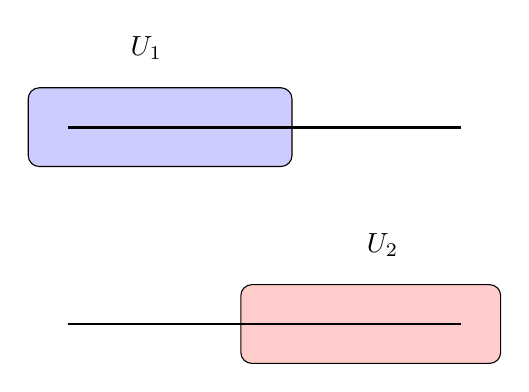
\begin{tikzpicture}

        \draw[rounded corners, fill=blue!20]  (-4,2) rectangle (-0.65,1);
        \draw[rounded corners, fill=red!20] (-1.3,-0.5) rectangle (2,-1.5);
        
        \draw[line width = 1pt] (-3.5,1.5) -- (1.5,1.5);
        \draw[line width = 1pt] (-3.5,-1) -- (1.5,-1);
        \node at (-2.5,2.5) {$U_1$};
        \node at (0.5,0) {$U_2$};
    \end{tikzpicture}\]
    Show that the map $i^*: C^1(X)\to C^2(X)$ is surjective, and so 
    \[ \dim(C^2(X))-\dim(\im(i^*))= \dim(\ker(0_{C^2(X)\to 0}))-\dim(\im(i^*))=0.\]
\end{exercise}
\begin{exercise}
    Let $X$ be the line segment, covered with $n$ open intervals which overlap as in the diagram below:
    \[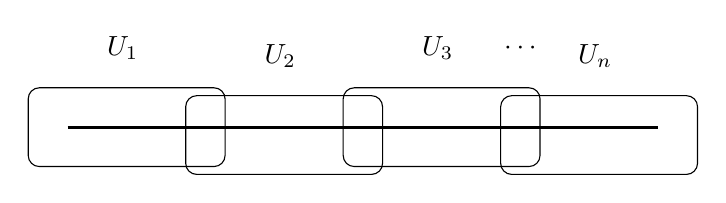
\begin{tikzpicture}

        \begin{scope}[]
        \draw[rounded corners]  (-4,2) rectangle (-1.5,1);
        \node at (-2.8,2.5) {$U_1$};
        \end{scope}\begin{scope}[shift={(4,0)}]
        \draw[rounded corners]  (-4,2) rectangle (-1.5,1);
        \node at (-2.8,2.5) {$U_3$};
        \end{scope}\begin{scope}[shift={(2,-0.1)}]
        \draw[rounded corners]  (-4,2) rectangle (-1.5,1);
        \node at (-2.8,2.5) {$U_2$};
        \end{scope}\begin{scope}[shift={(6,-0.1)}]
        \draw[rounded corners]  (-4,2) rectangle (-1.5,1);
        \node at (-2.8,2.5) {$U_n$};
        \end{scope}
        \draw[line width = 1pt] (-3.5,1.5) -- (4,1.5);
        \node at (2.25,2.5) {$\cdots$};
        \end{tikzpicture}
        \]
    Define a sequence 
    \[C^0(X)\xrightarrow{j^*}C^1(X)\xrightarrow{i^*}C^2(X)\]
    where $C^1(X)$ is based on the connected components of the $U_i$, and the $C^2(X)$ is based on the intersections $U_i\cap U_{i+1}$. 
    Again, show that 
    \[ \dim(C^2(X))-\dim(\im(i^*))= \dim(\ker(0_{C^2(X)\to 0}))-\dim(\im(i^*))=0.\]
\end{exercise}
\begin{exercise}
    Let $X$ be the circle, covered with $n$ intervals which overlap end to end as drawn below. 
    \[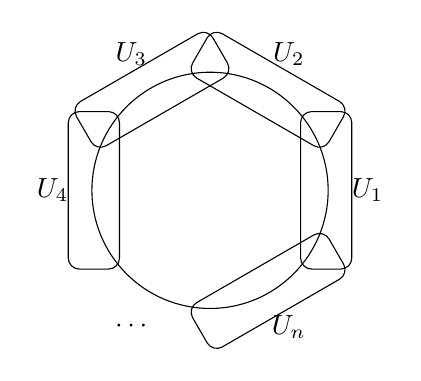
\begin{tikzpicture}
        \draw  (0,0) ellipse (1.5 and 1.5);
        \begin{scope}[]
        
        \draw[rounded corners]  (1.8,-1) rectangle (1.15,1);
        \node at (2,0) {$U_1$};
        \end{scope}
        \begin{scope}[rotate=60]
        
        \draw[rounded corners]  (1.8,-1) rectangle (1.15,1);
        \node at (2,0) {$U_2$};
        \end{scope}
        \begin{scope}[rotate=120]
        
        \draw[rounded corners]  (1.8,-1) rectangle (1.15,1);
        \node at (2,0) {$U_3$};
        \end{scope}
        \begin{scope}[rotate=180]
        
        \draw[rounded corners]  (1.8,-1) rectangle (1.15,1);
        \node at (2,0) {$U_4$};
        \end{scope}
        \begin{scope}[rotate=240]
        
        \node at (2,0) {$\cdots$};
        \end{scope}
        \begin{scope}[rotate=300]
        
        \draw[rounded corners]  (1.8,-1) rectangle (1.15,1);
        \node at (2,0) {$U_n$};
        \end{scope}
        \end{tikzpicture}\]
        Define $C^1(X)$ and $C^2(X)$ as in the previous problem.
        \begin{itemize}
        \item Pick a basis for $C^1(X)$ and $C^2(X)$ given by functions which map a single connected component to 1, and all other components to zero. Write down the map $i^*$ in this basis. 
        \item Show that for this cycle,
        \[ \dim(C^2(X))-\dim(\im(i^*))= \dim(\ker(0_{C^2(X)\to 0}))-\dim(\im(i^*))=-1.\]
        \end{itemize}
\end{exercise}
\begin{exercise}
    Cover this figure eight with sets so that
    \begin{itemize}
        \item Each set is connected 
        \item Each pair of sets intersect in one connected component
        \item No three sets have common overlap.
    \end{itemize}
\[    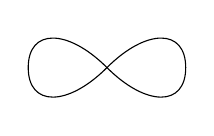
\begin{tikzpicture}
   \draw (-1,0.5) .. controls (-0.5,1) and (0,1) .. (0,0.5) .. controls (0,0) and (-0.5,0) .. (-1,0.5) .. controls (-1.5,1) and (-2,1) .. (-2,0.5) .. controls (-2,0) and (-1.5,0) .. (-1,0.5);
        \end{tikzpicture}\]
    Define a sequence 
    \[C^0(X)\xrightarrow{j^*}C^1(X)\xrightarrow{i^*}C^2(X)\]
    where $C^1(X)$ is based on the connected components of the $U_i$, and the $C^2(X)$ is based on intersection on the intersections $U_i\cap U_{k}$. 
    Then compute
    \[ \dim(\im(i^*))-\dim(C^2(X)).\]
\end{exercise}


\begin{exercise}
	Let $A^\bullet$ be a chain complex, and let $B^k:=H^k(A)$ be the chain complex whose cochain groups are given by the cohomology groups $H^k(A)$ and whose differential is always zero. 
	Verify that $\pi: A^\bullet\to B^\bullet$ which sends each element of $A$ to its cohomology class is a cochain map, and $\pi: H^k(A^\bullet)\to H^k(B^\bullet)$ is an isomorphism.
\end{exercise}
\begin{exercise}
	Let $X=(\Delta_X, \mathcal S_X)$ be a simplicial complex. A \emph{simplicial subcomplex} is a simplicial complex $Y=(\Delta_Y, \mathcal S_Y)$ with $\mathcal S_Y\subset \mathcal S_X$ and 
	\[\sigma\in \Delta_Y \Rightarrow \sigma\in \Delta_X.\]
	Show that if $Y$ is a subcomplex of $X$, there is a cochain map \[i^*: \underline C^\bullet(X, \ZZ_2)\to \underline C^\bullet(Y, \ZZ_2).\]
\end{exercise}
\begin{exercise}
	Let $Y\subset X$ be a simplicial subcomplex. 
	Denote the corresponding map of topological spaces $i: Y\to X$.
	Construct a new simplicial complex, $\cone(i)$ whose vertex set is  \[\mathcal S_{\cone}:= \mathcal S\cup\{x\},\]
	and whose simplifies are:
	\[\Delta_{\cone}:=\Delta_X\cup\{\sigma\cup\{x\}\;|\; \sigma \in \Delta_Y\}.\]
	Draw a picture for $\cone(i)$ when $X$ is an interval, and $Y$ is the two boundary vertices of the interval. 
	Furthermore, explain why this operation is called the cone.
\end{exercise}
\begin{exercise}
	Let $i^*:\underline C^\bullet(X, \ZZ_2)\to \underline C^\bullet(Y, \ZZ_2)$ be the map considered above. Prove that \[\underline C^\bullet(\cone(i), \ZZ_2 )=\cone^\bullet(i^*)[-1]\]
\end{exercise}
\begin{exercise}
	The $n$-disk  (denoted $D^n$) is the simplicial complex where $\mathcal S_{D^k}:=\{0, \ldots, n\}$ and 
	\[\Delta_{D^n}=\{\sigma \;|\; \sigma\subset \mathcal S_{D^n}\}.\]
	Let $\id_{D^n}: D^n\to D^n$ be the inclusion of $D^k$ into itself as a subcomplex. Show that 
	\[\cone(\id_{D^n})=D^{n+1}.\]
\end{exercise}
When $X$ is a simplicial complex, we denote by $H^i(X, \ZZ_2)$ to be the $i$-th cohomology group of $\underline C^\bullet(X, \ZZ_2)$.
\begin{exercise}
	Use the previous characterization of $D^{n+1}$ to compute the homology groups $\underline H^i(D^k)$ inductively. 
\end{exercise}
\begin{exercise}
	The $n$-sphere (denoted $S^n$) is the simplicial complex where ${\mathcal S}_{S^n}=\{0, \ldots, n+1\}$ and 
	\[\Delta_{S^n}=\{\sigma \;|\; \sigma\subset {\mathcal S}_{S^n}, \sigma \neq \{0, \ldots, n+1\}.\]
	Show that there is a map $i_{S^n}: S^n\to D^{n+1}$, and that 
	\[\cone(i_{S^n})=S^{n+1}.\]
\end{exercise}
\begin{exercise}
	Use the previous characterization of $S^{n+1}$ to compute the cohomology groups $\underline H^i(S^n)$ inductively. 
\end{exercise}

